\documentclass{standalone}
\usepackage{tikz}
\usetikzlibrary{patterns, positioning}


\begin{document}
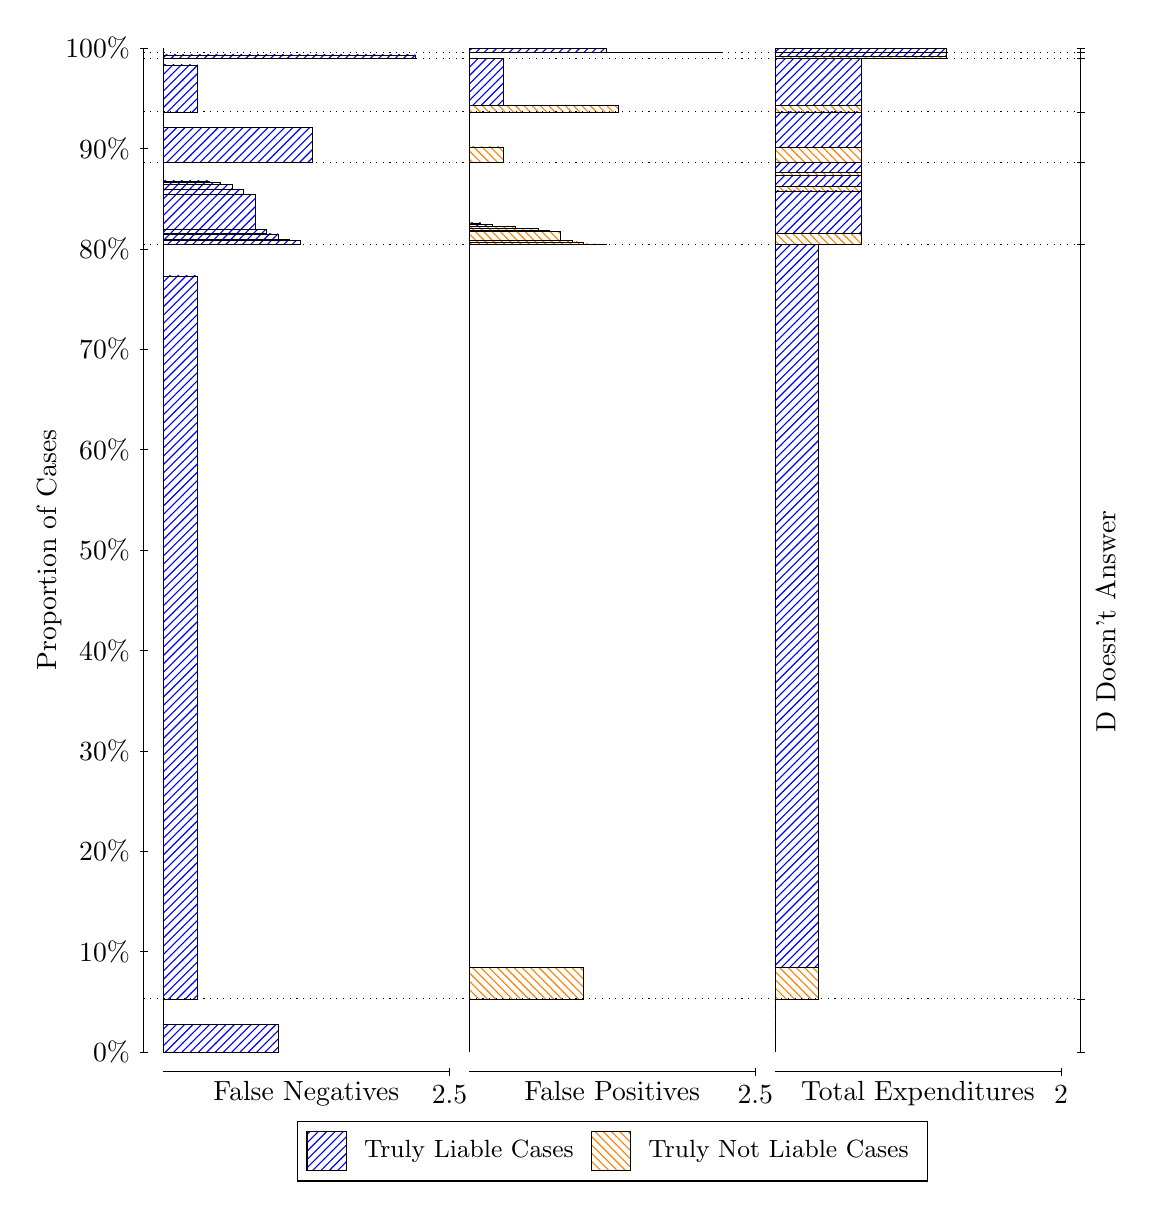
\begin{tikzpicture}
\draw[black, very thin] (1.5,1.75) -- (1.5,14.5);
\node[rotate=90, text=black, anchor=center] at (0.3, 8.125) {Proportion of Cases};
\draw[black, very thin] (1.45,1.75) -- (1.55,1.75);
\node[text=black, anchor=east] at (1.45, 1.75) {0\%};
\draw[black, very thin] (1.45,3.025) -- (1.55,3.025);
\node[text=black, anchor=east] at (1.45, 3.025) {10\%};
\draw[black, very thin] (1.45,4.3) -- (1.55,4.3);
\node[text=black, anchor=east] at (1.45, 4.3) {20\%};
\draw[black, very thin] (1.45,5.575) -- (1.55,5.575);
\node[text=black, anchor=east] at (1.45, 5.575) {30\%};
\draw[black, very thin] (1.45,6.85) -- (1.55,6.85);
\node[text=black, anchor=east] at (1.45, 6.85) {40\%};
\draw[black, very thin] (1.45,8.125) -- (1.55,8.125);
\node[text=black, anchor=east] at (1.45, 8.125) {50\%};
\draw[black, very thin] (1.45,9.4) -- (1.55,9.4);
\node[text=black, anchor=east] at (1.45, 9.4) {60\%};
\draw[black, very thin] (1.45,10.675) -- (1.55,10.675);
\node[text=black, anchor=east] at (1.45, 10.675) {70\%};
\draw[black, very thin] (1.45,11.95) -- (1.55,11.95);
\node[text=black, anchor=east] at (1.45, 11.95) {80\%};
\draw[black, very thin] (1.45,13.225) -- (1.55,13.225);
\node[text=black, anchor=east] at (1.45, 13.225) {90\%};
\draw[black, very thin] (1.45,14.5) -- (1.55,14.5);
\node[text=black, anchor=east] at (1.45, 14.5) {100\%};

\draw[black, very thin] (13.4,1.75) -- (13.4,14.5);
\draw[black, very thin] (13.35,1.75) -- (13.45,1.75);
\node[anchor=west] at (13.35, 1.75) {};
\draw[black, very thin] (13.35,2.4255) -- (13.45,2.4255);
\node[anchor=west] at (13.35, 2.4255) {};
\draw[black, very thin] (13.35,12.006) -- (13.45,12.006);
\node[anchor=west] at (13.35, 12.006) {};
\draw[black, very thin] (13.35,13.046) -- (13.45,13.046);
\node[anchor=west] at (13.35, 13.046) {};
\draw[black, very thin] (13.35,13.69) -- (13.45,13.69);
\node[anchor=west] at (13.35, 13.69) {};
\draw[black, very thin] (13.35,14.369) -- (13.45,14.369);
\node[anchor=west] at (13.35, 14.369) {};
\draw[black, very thin] (13.35,14.442) -- (13.45,14.442);
\node[anchor=west] at (13.35, 14.442) {};
\draw[black, very thin] (13.35,14.5) -- (13.45,14.5);
\node[anchor=west] at (13.35, 14.5) {};

\draw[black, very thin, pattern color=blue, pattern=north east lines] (1.75,1.75) rectangle (3.2033,2.0973);
\draw[black, very thin, pattern color=orange, pattern=north west lines] (1.75,2.0973) rectangle (1.75,2.4255);
\draw[black, very thin, pattern color=blue, pattern=north east lines] (1.75,2.4255) rectangle (2.186,11.606);
\draw[black, very thin, pattern color=orange, pattern=north west lines] (1.75,11.606) rectangle (1.75,12.006);
\draw[black, very thin, pattern color=blue, pattern=north east lines] (1.75,12.006) rectangle (3.494,12.054);
\draw[black, very thin, pattern color=blue, pattern=north east lines] (1.75,12.054) rectangle (3.3487,12.067);
\draw[black, very thin, pattern color=blue, pattern=north east lines] (1.75,12.067) rectangle (3.2033,12.141);
\draw[black, very thin, pattern color=blue, pattern=north east lines] (1.75,12.141) rectangle (3.058,12.148);
\draw[black, very thin, pattern color=blue, pattern=north east lines] (1.75,12.148) rectangle (3.058,12.196);
\draw[black, very thin, pattern color=blue, pattern=north east lines] (1.75,12.196) rectangle (2.9127,12.644);
\draw[black, very thin, pattern color=blue, pattern=north east lines] (1.75,12.644) rectangle (2.7673,12.701);
\draw[black, very thin, pattern color=blue, pattern=north east lines] (1.75,12.701) rectangle (2.622,12.772);
\draw[black, very thin, pattern color=blue, pattern=north east lines] (1.75,12.772) rectangle (2.4767,12.793);
\draw[black, very thin, pattern color=blue, pattern=north east lines] (1.75,12.793) rectangle (2.3313,12.814);
\draw[black, very thin, pattern color=orange, pattern=north west lines] (1.75,12.814) rectangle (1.75,13.046);
\draw[black, very thin, pattern color=blue, pattern=north east lines] (1.75,13.046) rectangle (3.6393,13.491);
\draw[black, very thin, pattern color=orange, pattern=north west lines] (1.75,13.491) rectangle (1.75,13.69);
\draw[black, very thin, pattern color=blue, pattern=north east lines] (1.75,13.69) rectangle (2.186,14.286);
\draw[black, very thin, pattern color=orange, pattern=north west lines] (1.75,14.286) rectangle (1.75,14.369);
\draw[black, very thin, pattern color=blue, pattern=north east lines] (1.75,14.369) rectangle (4.9473,14.413);
\draw[black, very thin, pattern color=orange, pattern=north west lines] (1.75,14.413) rectangle (1.75,14.442);
\draw[black, very thin, pattern color=orange, pattern=north west lines] (1.75,14.442) rectangle (1.75,14.447);
\draw[black, very thin, pattern color=blue, pattern=north east lines] (1.75,14.447) rectangle (1.75,14.5);
\draw[black, very thin, pattern color=orange, pattern=north west lines] (5.6333,1.75) rectangle (5.6333,2.0782);
\draw[black, very thin, pattern color=blue, pattern=north east lines] (5.6333,2.0782) rectangle (5.6333,2.4255);
\draw[black, very thin, pattern color=orange, pattern=north west lines] (5.6333,2.4255) rectangle (7.0867,2.8258);
\draw[black, very thin, pattern color=blue, pattern=north east lines] (5.6333,2.8258) rectangle (5.6333,12.006);
\draw[black, very thin, pattern color=orange, pattern=north west lines] (5.6333,12.006) rectangle (7.3773,12.009);
\draw[black, very thin, pattern color=orange, pattern=north west lines] (5.6333,12.009) rectangle (7.232,12.014);
\draw[black, very thin, pattern color=orange, pattern=north west lines] (5.6333,12.014) rectangle (7.0867,12.037);
\draw[black, very thin, pattern color=orange, pattern=north west lines] (5.6333,12.037) rectangle (6.9413,12.056);
\draw[black, very thin, pattern color=orange, pattern=north west lines] (5.6333,12.056) rectangle (6.796,12.167);
\draw[black, very thin, pattern color=orange, pattern=north west lines] (5.6333,12.167) rectangle (6.6507,12.184);
\draw[black, very thin, pattern color=orange, pattern=north west lines] (5.6333,12.184) rectangle (6.5053,12.207);
\draw[black, very thin, pattern color=orange, pattern=north west lines] (5.6333,12.207) rectangle (6.36,12.214);
\draw[black, very thin, pattern color=orange, pattern=north west lines] (5.6333,12.214) rectangle (6.2147,12.237);
\draw[black, very thin, pattern color=blue, pattern=north east lines] (5.6333,12.237) rectangle (5.924,12.259);
\draw[black, very thin, pattern color=blue, pattern=north east lines] (5.6333,12.259) rectangle (5.7787,12.279);
\draw[black, very thin, pattern color=blue, pattern=north east lines] (5.6333,12.279) rectangle (5.6333,13.046);
\draw[black, very thin, pattern color=orange, pattern=north west lines] (5.6333,13.046) rectangle (6.0693,13.244);
\draw[black, very thin, pattern color=blue, pattern=north east lines] (5.6333,13.244) rectangle (5.6333,13.69);
\draw[black, very thin, pattern color=orange, pattern=north west lines] (5.6333,13.69) rectangle (7.5227,13.773);
\draw[black, very thin, pattern color=blue, pattern=north east lines] (5.6333,13.773) rectangle (6.0693,14.369);
\draw[black, very thin, pattern color=orange, pattern=north west lines] (5.6333,14.369) rectangle (5.6333,14.398);
\draw[black, very thin, pattern color=blue, pattern=north east lines] (5.6333,14.398) rectangle (5.6333,14.442);
\draw[black, very thin, pattern color=orange, pattern=north west lines] (5.6333,14.442) rectangle (8.8307,14.447);
\draw[black, very thin, pattern color=blue, pattern=north east lines] (5.6333,14.447) rectangle (7.3773,14.5);
\draw[black, very thin, pattern color=orange, pattern=north west lines] (9.5167,1.75) rectangle (9.5167,2.0782);
\draw[black, very thin, pattern color=blue, pattern=north east lines] (9.5167,2.0782) rectangle (9.5167,2.4255);
\draw[black, very thin, pattern color=orange, pattern=north west lines] (9.5167,2.4255) rectangle (10.062,2.8258);
\draw[black, very thin, pattern color=blue, pattern=north east lines] (9.5167,2.8258) rectangle (10.062,12.006);
\draw[black, very thin, pattern color=orange, pattern=north west lines] (9.5167,12.006) rectangle (10.607,12.145);
\draw[black, very thin, pattern color=blue, pattern=north east lines] (9.5167,12.145) rectangle (10.607,12.686);
\draw[black, very thin, pattern color=orange, pattern=north west lines] (9.5167,12.686) rectangle (10.607,12.742);
\draw[black, very thin, pattern color=blue, pattern=north east lines] (9.5167,12.742) rectangle (10.607,12.885);
\draw[black, very thin, pattern color=orange, pattern=north west lines] (9.5167,12.885) rectangle (10.607,12.921);
\draw[black, very thin, pattern color=blue, pattern=north east lines] (9.5167,12.921) rectangle (10.607,13.046);
\draw[black, very thin, pattern color=orange, pattern=north west lines] (9.5167,13.046) rectangle (10.607,13.244);
\draw[black, very thin, pattern color=blue, pattern=north east lines] (9.5167,13.244) rectangle (10.607,13.69);
\draw[black, very thin, pattern color=orange, pattern=north west lines] (9.5167,13.69) rectangle (10.607,13.773);
\draw[black, very thin, pattern color=blue, pattern=north east lines] (9.5167,13.773) rectangle (10.607,14.369);
\draw[black, very thin, pattern color=orange, pattern=north west lines] (9.5167,14.369) rectangle (11.697,14.398);
\draw[black, very thin, pattern color=blue, pattern=north east lines] (9.5167,14.398) rectangle (11.697,14.442);
\draw[black, very thin, pattern color=orange, pattern=north west lines] (9.5167,14.442) rectangle (11.697,14.447);
\draw[black, very thin, pattern color=blue, pattern=north east lines] (9.5167,14.447) rectangle (11.697,14.5);
\draw[black, dotted] (1.5,2.4255) -- (13.4,2.4255);
\draw[black, dotted] (1.5,12.006) -- (13.4,12.006);
\draw[black, dotted] (1.5,13.046) -- (13.4,13.046);
\draw[black, dotted] (1.5,13.69) -- (13.4,13.69);
\draw[black, dotted] (1.5,14.369) -- (13.4,14.369);
\draw[black, dotted] (1.5,14.442) -- (13.4,14.442);
\draw[black, very thin] (1.75,1.5) -- (5.3833,1.5);
\node[text=black, anchor=north] at (3.5667, 1.5) {False Negatives};
\draw[black, very thin] (5.3833,1.45) -- (5.3833,1.55);
\node[text=black, anchor=north] at (5.3833, 1.45) {2.5};

\draw[black, very thin] (5.6333,1.5) -- (9.2667,1.5);
\node[text=black, anchor=north] at (7.45, 1.5) {False Positives};
\draw[black, very thin] (9.2667,1.45) -- (9.2667,1.55);
\node[text=black, anchor=north] at (9.2667, 1.45) {2.5};

\draw[black, very thin] (9.5167,1.5) -- (13.15,1.5);
\node[text=black, anchor=north] at (11.333, 1.5) {Total Expenditures};
\draw[black, very thin] (13.15,1.45) -- (13.15,1.55);
\node[text=black, anchor=north] at (13.15, 1.45) {2};


\node[text=black, centered, rotate=90] at (13.72, 7.2157) {D Doesn't Answer};






\draw (7.449999999999999,1.5) node[draw=none] (baseCoordinate) {};
\begin{scope}[align=center]
        \matrix[scale=0.5, draw=black, below=0.5cm of baseCoordinate, nodes={draw}, column sep=0.1cm]{
            \node[rectangle, draw, minimum width=0.5cm, minimum height=0.5cm, pattern color=blue, pattern=north east lines] {}; &
            \node[draw=none, font=\small, text=black] (B) {Truly Liable Cases}; &
            \node[rectangle, draw, minimum width=0.5cm, minimum height=0.5cm, pattern color=orange, pattern=north west lines] {}; &
            \node[draw=none, font=\small, text=black] (B) {Truly Not Liable Cases}; \\
            };
\end{scope}

\end{tikzpicture}
\end{document}